%%%%%%%%%%%%%%%%%%%%%%%%%%%%%%%%%%%%%%%%%%%%%%
%                                            %
%   W Z O R Z E C   S P R A W O Z D A N I A  %
%                                            %
%%%%%%%%%%%%%%%%%%%%%%%%%%%%%%%%%%%%%%%%%%%%%%


\documentclass[12pt,a4paper,twoside]{article}

\usepackage{amsmath,amssymb}
\usepackage[utf8]{inputenc}                                      
\usepackage[OT4]{fontenc}      
%\usepackage[T1]{fontenc}                            
\usepackage[polish]{babel}                           
\selectlanguage{polish}
\usepackage{indentfirst} 
\usepackage[dvips]{graphicx}
\usepackage{tabularx}
\usepackage{color}
\usepackage{hyperref} 
\usepackage{fancyhdr}
\usepackage{listings}
\usepackage{booktabs}
\usepackage{ifpdf}
\usepackage{mathtext} % polskie znaki w trybie matematycznym
%\makeindex  % utworzenie skorowidza (w dokumencie pdf)
\usepackage{lmodern}
%\usepackage[osf]{libertine}
\usepackage{filecontents}
\usepackage{ifthen}


\usepackage{tikz}
\usetikzlibrary{arrows}


\newcounter{nextYear}
\setcounter{nextYear}{\the\year}
\stepcounter{nextYear}

% rozszerzenie nieco strony
%\setlength{\topmargin}{-1cm} \setlength{\textheight}{24.5cm}
%\setlength{\textwidth}{17cm} \addtolength{\hoffset}{-1.5cm}
%\setlength{\parindent}{0.5cm} \setlength{\footskip}{2cm}
%\linespread{1.2} % odstep pomiedzy wierszami


%%%% ZYWA PAGINA %%%%%%%%%%%
\newcommand{\tl}[1]{\textbf{#1}} 
\pagestyle{fancy}
\renewcommand{\sectionmark}[1]{\markright{\thesection\ #1}}
\fancyhf{} % usuwanie bieżących ustawień
\fancyhead[LE,RO]{\small\bfseries\thepage}
\fancyhead[LO]{\small\bfseries\rightmark}
\fancyhead[RE]{\small\bfseries\leftmark}
\renewcommand{\headrulewidth}{0.5pt}
\renewcommand{\footrulewidth}{0pt}
\addtolength{\headheight}{0.5pt} % pionowy odstęp na kreskę
\fancypagestyle{plain}{%
\fancyhead{} % usuń p. górne na stronach pozbawionych numeracji
\renewcommand{\headrulewidth}{0pt} % pozioma kreska
}

%%%%%   LISTINGI %%%%%%%%
% ustawienia listingu programow

\lstset{%
language=C++,%
commentstyle=\textit,%
identifierstyle=\textsf,%
keywordstyle=\sffamily\bfseries, %
%captionpos=b,%
tabsize=3,%
frame=lines,%
numbers=left,%
numberstyle=\tiny,%
numbersep=5pt,%
breaklines=true,%
morekeywords={pWezel,Wezel,string,ref,params_result},%
escapeinside={(*@}{@*)},%
%basicstyle=\footnotesize,%
%keywords={double,int,for,if,return,vector,matrix,void,public,class,string,%
%float,sizeof,char,FILE,while,do,const}
}
%%%%%%%%%%%%%%%%%%%%%%%%%%%%%%%%%%%%%%%%%%%%%%%%%%%%%%%%%%%%%%%%%%%%%%%

%%%%%%%%%  NOTKI NA MARGINESIE %%%%%%%%%%%%%
% mala zmiana sposobu wyswietlania notek bocznych
\let\oldmarginpar\marginpar
\renewcommand\marginpar[1]{%
  {\linespread{0.85}\normalfont\scriptsize%
\oldmarginpar[\hspace{1cm}\begin{minipage}{3cm}\raggedleft\scriptsize\color{black}\textsf{#1}\end{minipage}]%    left pages
{\hspace{0cm}\begin{minipage}{3cm}\raggedright\scriptsize\color{black}\textsf{#1}\end{minipage}}% right pages
}%
}
% % % % % % % % % % % % % % % % % % % % % % % % % % % % % % % %

%%%% WYSWIETLANIE AKTUALNEGO ROKU AKADEMICKIEGO %%%%%%%%%%%
\newcounter{rok}
\newcommand{\rokakademicki}{%
   \setcounter{rok}{\number\year}%
   \ifthenelse{\number\month<10}%
   {\addtocounter{rok}{-1}}% rok akademicki zaczal sie w pazdzierniku poprzedniego roku
   {}%                       rok akademicki zaczyna sie w pazdzierniku tego roku
   \arabic{rok}/\addtocounter{rok}{1}\arabic{rok}
}
%%%%%%%%%%%%%%%%%%%%%%%%%%%%%%%%%%%%%%%


%%%% LISTA UWAG %%%%%%%%%
\usepackage{color}
\definecolor{brickred}      {cmyk}{0   , 0.89, 0.94, 0.28}

\makeatletter \newcommand \kslistofremarks{\section*{Uwagi} \@starttoc{rks}}
\newcommand\l@uwagas[2]
{\par\noindent \textbf{#2:} %\parbox{10cm}
   {#1}\par} \makeatother


\newcommand{\ksremark}[1]{%
   {{\color{brickred}{[#1]}}}%
   \addcontentsline{rks}{uwagas}{\protect{#1}}%
}

\newcommand{\comma}{\ksremark{przecinek}}
\newcommand{\nocomma}{\ksremark{bez przecinka}}
\newcommand{\styl}{\ksremark{styl}}
\newcommand{\ortografia}{\ksremark{ortografia}}
\newcommand{\fleksja}{\ksremark{fleksja}}
\newcommand{\pauza}{\ksremark{pauza `--', nie dywiz `-'}}
\newcommand{\kolokwializm}{\ksremark{kolokwializm}}
\newcommand{\cytowanie}{\ksremark{cytowanie}}

%%%%%%%%%%%%%%%%%%%%%%%%%
%%%%%%%%%%%%%%%%%%%%%%%%%
%%%%%%%%%%%%%%%%%%%%%%%%%
%%%%%%%%%%%%%%%%%%%%%%%%%
%%%%%%%%%%%%%%%%%%%%%%%%%
%%%%%%%%%%%%%%%%%%%%%%%%%
%%%%%%%%%%%%%%%%%%%%%%%%%
%%%%%%%%%%%%%%%%%%%%%%%%%
%%%%%%%%%%%%%%%%%%%%%%%%%
%%%%%%%%%%%%%%%%%%%%%%%%%
%%%%%%%%%%%%%%%%%%%%%%%%%
%%%%%%%%%%%%%%%%%%%%%%%%%



% autor:
\fancyhead[RE]{\small\bfseries Hanna Podeszwa} % autor sprawozdania



%%%%%%%%%%% NO I ZACZYNA SIE SPRAWOZDANIE %%%%%%%%%%%

\begin{document}
\frenchspacing
\thispagestyle{empty}
\begin{center}
{\Large\sf Politechnika Śląska   % Alma Mater

Wydział Automatyki, Elektroniki i Informatyki

}

\vfill

 

\vfill\vfill

{\Huge\sffamily\bfseries Podstawy Programowania Komputerów\par}  

\vfill\vfill

{\LARGE\sf Spedycja}   


\vfill \vfill\vfill\vfill

%%%%%%%%%%%%%%%%%%%%%%%%%%%%





\begin{tabular}{ll}
	\toprule
	autor                       & Hanna Podeszwa     \\
	prowadzący                  & dr inż. Krzysztof Simiński  \\
	rok akademicki              & 2018/2019         \\
	kierunek                    & informatyka            \\
	rodzaj studiów              & SSI                    \\
	semestr                     & 1                      \\
	termin laboratorium         & środa, 13:45 -- 15:15 \\
	sekcja                      & 18                     \\
	termin oddania sprawozdania & 2019-01-11             \\
	\bottomrule
	                            &
\end{tabular}

\end{center}
%%% koniec strony  tytulowej

%%%%%%%%%%%%%%%%%%%%%%%%%%%%%%%%%%%%%%%%%%%%%%%%%%%%%%%%%%%%%%%%%%%%%%%%%
\cleardoublepage
%%%%%%%%%%%%%%%%%%%%%%%%%%%%%%%%%%%%%%%%%%%%%%%%%%%%%%%%%%%%%%%%%%%%%%%%%

%%%%%%%%%%%%%%%%%%%%%%%%%%%%%%%%%%%%%%%%%%%%%%%%%%%%%%%%%%%%%%%%%%%%%%%%%
\section{Treść zadania}

Napisać program wyszukujący najkrótsze możliwe trasy spedycyjne, wykorzystując algorytm Dijkstry. Miasta sąsiednie wraz z odległościami między nimi są zawarte w pliku tekstowym. Każda para miast jest w osobnej linii. Najkrótsze trasy spedycyjne zostaną zapisane do pliku, począwszy od miasta startowego, poprzez miasta sąsiednie (każda trasa w osobnej linii).

Program uruchamiany jest z linii poleceń z wykorzystaniem następujących przełączników:
 
\begin{tabular}{ll}
\texttt{-i}  & plik wejściowy z sąsiednimi miastami i odległościami między nimi\\
\texttt{-o}  & plik wyjściowy z trasami spedycyjnymi\\
\texttt{-s}  & miasto startowe\\
\end{tabular}

%%%%%%%%%%%%%%%%%%%%%%%%%%%%%%%%%%%%%%%%%%%%%%%%%%%%%%%%%%%%%%%%%%%%%%%%%
\section{Analiza zadania}

Zagadnienie przedstawia problem znalezienia najkrótszej możliwej trasy spedycyjnej pomiędzy miastem startowym, a wszystkimi innymi miastami zapisanymi w pliku.

\subsection{Struktury danych}

W programie wykorzystano listy jednokierunkowe do przechowywania miasta i dróg. Każdy element listy miast zawiera trzy wskaźniki: na nastepny element listy miast, na listę dróg oraz na miasto poprzednie, nazwę miasta, odległość od centrali oraz informację, czy dane miasto zostało już odwiedzone. Elementy listy dróg zawierają wskaźnik na odpowiednie miasto z listy miast oraz odległość między tym miastem, a miastem poprzednim.
Rysunek \ref{fig:listy} przedstawia przykład . 
Taka struktura danych umożliwia łatwe zastosowanie algorytmu Dijkstry.


\subsection{Algorytmy}

Program  wyszukuje najkrótsze możliwe trasy spedycyjne, wykorzystując algorytm Dijkstry.
Zaczynając zawsze od miasta położonego najbliżej miasta startowego, porównuje wartość sumy wartości zmiennej \lstinline!odleglosc_od_centrali! poprzedniego miasta i odległości między tymi miastami z aktualną wartością zmiennej \lstinline!odleglosc_od_centrali! miasta następnego. Kolejnym krokiem jest relaksacja odległości od centrali wraz z ewentualnym zapamiętaniem adresu miasta poprzedniego.
Utworzenie list i ich przejście jest wykonywane w średnim czasie $O(n^2+m)$ (gdzie n oznacza ilość elementów listy miast, a m ilość elementów list dróg).
%\marginpar{Tutaj można umieścić wzory, które są wykorzystane w implementacji:
%\begin{equation}\label{eq:rownanie}
%S = \sum^\infty_{n = 0} \frac{1}{n!}e^{n\omega j}.
%\end{equation}
%}



\begin{figure}
\centering
\begin{tikzpicture}
\ %draw [help lines] grid (6,6);
\node[circle, draw] (A) at (-2,8) {$n1$};
\node[circle, draw] (B) at (-2,6) {$n2$};
\node[circle, draw] (C) at (-2,4) {$n3$};
\node[circle, draw] (D) at (-2,2) {$n.$};
\node[circle, draw] (E) at (-2,0) {$nn$};
\node[circle, draw] (F) at (2,8) {$m11$};
\node[circle, draw] (G) at (4,8) {$m12$};
\node[circle, draw] (H) at (6,8) {$m13$};
\node[circle, draw] (I) at (2,6) {$m21$};
\node[circle, draw] (J) at (4,6) {$m22$};
\node[circle, draw] (K) at (2,4) {$m31$};
\node[circle, draw] (L) at (4,4) {$m32$};
\node[circle, draw] (M) at (6,4) {$m33$};
\node[circle, draw] (N) at (8,4) {$m34$};
\node[circle, draw] (O) at (2,2) {$m.1$};
\node[circle, draw] (P) at (4,7) {$ $};
\node[circle, draw] (R) at (6,7) {$ $};
\node[circle, draw] (S) at (4,3) {$ $};
\node[circle, draw] (T) at (6,3) {$ $};
\node[circle, draw] (U) at (8,3) {$ $};

\draw[>=latex,->] (G) -- (P);
\draw[>=latex,->] (R) -- (H);
\draw[>=latex,->] (I) -- (A);
\draw[>=latex,->] (J) -- (D);
\draw[>=latex,->] (K) -- (B);
\draw[>=latex,->] (L) -- (S);
\draw[>=latex,->] (A) -- (B);
\draw[>=latex,->] (B) -- (C);
\draw[>=latex,->] (C) -- (D);
\draw[>=latex,->] (D) -- (E);
\draw[>=latex,->] (A) -- (F);
\draw[>=latex,->] (F) -- (G);
\draw[>=latex,->] (F) -- (C);
\draw[>=latex,->] (I) -- (J);
\draw[>=latex,->] (B) -- (I);
\draw[>=latex,->] (C) -- (K);
\draw[>=latex,->] (K) -- (L);
\draw[>=latex,->] (L) -- (M);
\draw[>=latex,->] (M) -- (N);
\draw[>=latex,->] (D) -- (O);
\draw[>=latex,->] (O) -- (A);
\draw[>=latex,->] (M) -- (T);
\draw[>=latex,->] (N) -- (U);
\draw[>=latex,->] (G) -- (H);


\end{tikzpicture}
\caption{Przykład listy miast i listy dróg.}
\label{fig:listy}
\end{figure} 

%%%%%%%%%%%%%%%%%%%%%%%%%%%%%%%%%%%%%%%%%%%%%%%%%%%%%%%%%%%%%%%%%%%%%%%%%
\section{Specyfikacja zewnętrzna}
\label{sec:sp:zewnetrzna}
Program jest uruchamiany z linii poleceń. 

Należy przekazać do programu nazwy plików: wejściowego i wyjściowego oraz nazwę miasta startowego po odpowiednich przełącznikach (odpowiednio: \texttt{-i} dla pliku wejściowego, \texttt{-o} dla pliku wyjściowego i \texttt{-s} dla miasta startowego), np.
\begin{verbatim}
program -i miasta.txt -o trasy -s startowe
program -o trasy -s startowe -i miasta.txt 
\end{verbatim}
Pliki są plikami tekstowymi, ale mogą mieć dowolne rozszerzenie (lub go nie mieć.) Przełączniki mogą być podane w dowolnej kolejności. Uruchomienie programu bez żadnego parametru lub z parametrem \texttt{-h}
\begin{verbatim}
program 
program -h
\end{verbatim}
powoduje wyświetlenie krótkiej pomocy. Uruchomienie programu z nieprawidłowymi parametrami powoduje wyświetlenie komunikatu 
\begin{verbatim}
Bledne argumenty
\end{verbatim}
i wyświetlenie pomocy. 

Podanie nieprawidłowej nazwy pliku powoduje wyświetlenie odpowiedniego komunikatu:
\begin{verbatim}
Nie udalo sie otworzyc pliku.
\end{verbatim}


%%%%%%%%%%%%%%%%%%%%%%%%%%%%%%%%%%%%%%%%%%%%%%%%%%%%%%%%%%%%%%%%%%%%%%%%%
\section{Specyfikacja wewnętrzna}\label{sec:sp-wew}
 Program został zrealizowany zgodnie z paradygmatem strukturalnym.  
W~programie rozdzielono interfejs (komunikację z użytkownikiem) od logiki aplikacji (sortowania liczb).


\subsection{Ogólna struktura programu}

W funkcji głównej wywołana jest funkcja \lstinline|sprawdzArgumenty|.
Funkcja ta sprawdza, czy program został wywołany w prawidłowy sposób. Gdy program nie został wywołany prawidłowo, zostaje wypisany stosowny komunikat i program się kończy.
Następnie wywoływana jest funkcja \lstinline|wczytajzPliku|.
Funkcja ta otwiera plik wejściowy, sczytuje miasta oraz odległości między nimi i umieszcza je w odpowiednich listach jednokierunkowych.
Po sczytaniu wszystkich miast funkcja zamyka plik.
W razie wystąpienia błędu funkcja zwraca \lstinline!false!, w przeciwnym wypadku \lstinline!true!.
Następnie wywoływana jest funkcja \lstinline|Dijkstra|.
Funkcja przechodzi przez listy i zapisuje odpowiednie wartosci w zmiennych \lstinline!odleglosc_od_centrali! i \lstinline!pMiastoPoprzednie!.
Następnie wywoływana jest funkcja \lstinline|wypisz_wynik|.Funkcja zapisuje trasy spedycyjne i odległości od centrali do pliku wyjściowego. Po zapisaniu tras funkcja zamyka plik.
Ostatnią funkcją programu jest funkcja \lstinline|usun| zwalniająca pamięć.


\subsection{Szczegółowy opis typów i funkcji}

Szczegółowy opis typów i funkcji zawarty jest w załączniku.

 

\section{Testowanie}

Program został przetestowany na różnego rodzaju plikach. Pliki niepoprawne (zawierające zbyt małą ilość miast lub niezawierające odległości) powodują zgłoszenie błędu. Plik pusty nie powoduje zgłoszenia błędu, ale utworzenie pustego pliku wynikowego (nie zostały podane żadne miasta ani odległości). 

Program został sprawdzony pod kątem wycieków pamięci.

%\section{Uzyskane wyniki}
%Jeżeli zadanie tego wymaga, wyniki można przestawić w~różny sposób, np. w tabeli ({\it vide} tabela \ref{tab:1}), czy na~rysunku ({\it vide} rycina \ref{fig:rysunek}) albo po prostu opisać uzyskane wyniki.
%



\section{Wnioski}

Program, wyszukujący najkrótsze możliwe trasy spedycyjne, jest programem prostym, chociaż wymaga samodzielnego zarządzania pamięcią. Najbardziej wymagające okazało się zastosowanie algorytmy Dijkstry. Szczególnie trudne było zapewnienie wpisywania prawidłowych wartości do zmiennej \lstinline!odleglosc_od_centrali!, tak by wypisane trasy spedycyjne były możliwie najkrótsze. Przygotowanie tego projektu pozwoliło mi lepiej zrozumieć sposób działania list jednokierunkowych oraz wskaźników.

%\begin{figure}[t]
%\centering
%\includegraphics{graf/rysunek.1}
%\caption{Opis rysunku znajduje się pod nim.}
%\label{fig:rysunek}
%\end{figure}


 

\begin{filecontents}{bibliografia.bib}
@article{Oetiker2007NieZaKrotkie,
	author       = {Tobias Oetiker and Tomasz Przechlewski and Ryszard Kubiak},
	title       = {Nie za kr\'{o}tkie wprowadzenie do systemu {L}a{T}e{X}2e}},
	YEAR         = {2007},


@ARTICLE{id:Abonyi2002modifiedgathgevafuzzy,
  author = {Abonyi, J\'{a}nos and Babu\v{s}ka, Robert and Szeifert, Ferenc},
  title = {{Modified Gath-Geva fuzzy clustering for identification of Takagi-Sugeno
	fuzzy models}},
  journal = {Systems, Man, and Cybernetics, Part B, IEEE Transactions on},
  year = {2002},
  volume = {32},
  pages = {612--621},
  number = {5}
}

@BOOK{
  title = {C++. Algorytmy i struktury danych},
  publisher = {Helion},
  year = {2001},
  author = {Adam Drozdek},
  address = {Gliwice}
}
@BOOK{
	title = {Podstawy algorytm\'{o}w z przykładami w C++},
	publisher = {Helion},
	year = {2004},
	author = {Richard Neapolitan, Kumarss Naimipour},
	address = {Gliwice}
}
\end{filecontents}


\bibliographystyle{plplain}
\bibliography{bibliografia}

%\pagebreak

 
\cleardoublepage

\rule{0cm}{0cm}

\vfill

\begin{center}
\Huge\bfseries Dodatek\\Szczegółowy opis typów i~funkcji\par
\end{center}
\documentclass[twoside]{book}

% Packages required by doxygen
\usepackage{fixltx2e}
\usepackage{calc}
\usepackage{doxygen}
\usepackage[export]{adjustbox} % also loads graphicx
\usepackage{graphicx}
\usepackage[utf8]{inputenc}
\usepackage{makeidx}
\usepackage{multicol}
\usepackage{multirow}
\PassOptionsToPackage{warn}{textcomp}
\usepackage{textcomp}
\usepackage[nointegrals]{wasysym}
\usepackage[table]{xcolor}

% Font selection
\usepackage[T1]{fontenc}
\usepackage[scaled=.90]{helvet}
\usepackage{courier}
\usepackage{amssymb}
\usepackage{sectsty}
\renewcommand{\familydefault}{\sfdefault}
\allsectionsfont{%
  \fontseries{bc}\selectfont%
  \color{darkgray}%
}
\renewcommand{\DoxyLabelFont}{%
  \fontseries{bc}\selectfont%
  \color{darkgray}%
}
\newcommand{\+}{\discretionary{\mbox{\scriptsize$\hookleftarrow$}}{}{}}

% Page & text layout
\usepackage{geometry}
\geometry{%
  a4paper,%
  top=2.5cm,%
  bottom=2.5cm,%
  left=2.5cm,%
  right=2.5cm%
}
\tolerance=750
\hfuzz=15pt
\hbadness=750
\setlength{\emergencystretch}{15pt}
\setlength{\parindent}{0cm}
\setlength{\parskip}{3ex plus 2ex minus 2ex}
\makeatletter
\renewcommand{\paragraph}{%
  \@startsection{paragraph}{4}{0ex}{-1.0ex}{1.0ex}{%
    \normalfont\normalsize\bfseries\SS@parafont%
  }%
}
\renewcommand{\subparagraph}{%
  \@startsection{subparagraph}{5}{0ex}{-1.0ex}{1.0ex}{%
    \normalfont\normalsize\bfseries\SS@subparafont%
  }%
}
\makeatother

% Headers & footers
\usepackage{fancyhdr}
\pagestyle{fancyplain}
\fancyhead[LE]{\fancyplain{}{\bfseries\thepage}}
\fancyhead[CE]{\fancyplain{}{}}
\fancyhead[RE]{\fancyplain{}{\bfseries\leftmark}}
\fancyhead[LO]{\fancyplain{}{\bfseries\rightmark}}
\fancyhead[CO]{\fancyplain{}{}}
\fancyhead[RO]{\fancyplain{}{\bfseries\thepage}}
\fancyfoot[LE]{\fancyplain{}{}}
\fancyfoot[CE]{\fancyplain{}{}}
\fancyfoot[RE]{\fancyplain{}{\bfseries\scriptsize Generated by Doxygen }}
\fancyfoot[LO]{\fancyplain{}{\bfseries\scriptsize Generated by Doxygen }}
\fancyfoot[CO]{\fancyplain{}{}}
\fancyfoot[RO]{\fancyplain{}{}}
\renewcommand{\footrulewidth}{0.4pt}
\renewcommand{\chaptermark}[1]{%
  \markboth{#1}{}%
}
\renewcommand{\sectionmark}[1]{%
  \markright{\thesection\ #1}%
}

% Indices & bibliography
\usepackage{natbib}
\usepackage[titles]{tocloft}
\setcounter{tocdepth}{3}
\setcounter{secnumdepth}{5}
\makeindex

% Hyperlinks (required, but should be loaded last)
\usepackage{ifpdf}
\ifpdf
  \usepackage[pdftex,pagebackref=true]{hyperref}
\else
  \usepackage[ps2pdf,pagebackref=true]{hyperref}
\fi
\hypersetup{%
  colorlinks=true,%
  linkcolor=blue,%
  citecolor=blue,%
  unicode%
}

% Custom commands
\newcommand{\clearemptydoublepage}{%
  \newpage{\pagestyle{empty}\cleardoublepage}%
}

\usepackage{caption}
\captionsetup{labelsep=space,justification=centering,font={bf},singlelinecheck=off,skip=4pt,position=top}

%===== C O N T E N T S =====

\begin{document}

% Titlepage & ToC
\hypersetup{pageanchor=false,
             bookmarksnumbered=true,
             pdfencoding=unicode
            }
\pagenumbering{alph}
\begin{titlepage}
\vspace*{7cm}
\begin{center}%
{\Large My Project }\\
\vspace*{1cm}
{\large Generated by Doxygen 1.8.14}\\
\end{center}
\end{titlepage}
\clearemptydoublepage
\pagenumbering{roman}
\tableofcontents
\clearemptydoublepage
\pagenumbering{arabic}
\hypersetup{pageanchor=true}

%--- Begin generated contents ---
\chapter{Class Index}
\section{Class List}
Here are the classes, structs, unions and interfaces with brief descriptions\+:\begin{DoxyCompactList}
\item\contentsline{section}{\mbox{\hyperlink{structdroga}{droga}} }{\pageref{structdroga}}{}
\item\contentsline{section}{\mbox{\hyperlink{structmiasto}{miasto}} }{\pageref{structmiasto}}{}
\item\contentsline{section}{\mbox{\hyperlink{structwynik}{wynik}} }{\pageref{structwynik}}{}
\end{DoxyCompactList}

\chapter{Class Documentation}
\hypertarget{structdroga}{}\section{droga Struct Reference}
\label{structdroga}\index{droga@{droga}}


{\ttfamily \#include $<$struktury.\+h$>$}



Collaboration diagram for droga\+:
\nopagebreak
\begin{figure}[H]
\begin{center}
\leavevmode
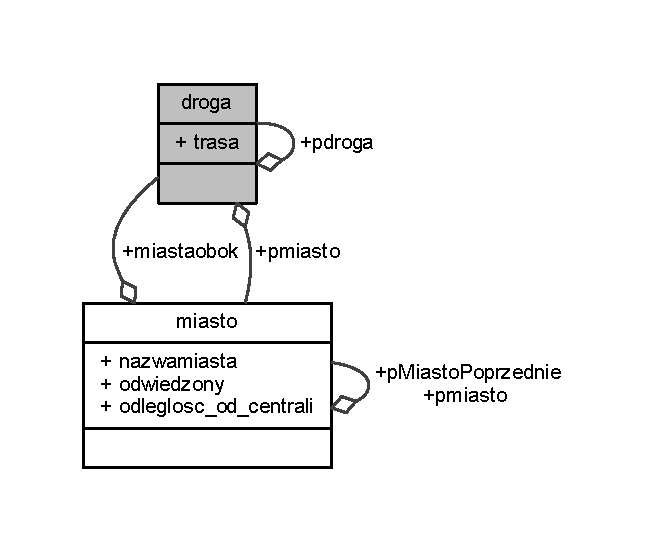
\includegraphics[width=310pt]{structdroga__coll__graph}
\end{center}
\end{figure}
\subsection*{Public Attributes}
\begin{DoxyCompactItemize}
\item 
int \mbox{\hyperlink{structdroga_a4788083344d3da2783792f80b35ab524}{trasa}}
\item 
\mbox{\hyperlink{structdroga}{droga}} $\ast$ \mbox{\hyperlink{structdroga_a7ed57ce3de3b4184ba7f7c805964626f}{pdroga}}
\item 
\mbox{\hyperlink{structmiasto}{miasto}} $\ast$ \mbox{\hyperlink{structdroga_a9c782b9f5281ee0f4cb4581a364b4471}{pmiasto}}
\end{DoxyCompactItemize}


\subsection{Detailed Description}
Struktura droga 
\begin{DoxyParams}{Parameters}
{\em trasa} & odleglosc miedzy miastami \\
\hline
{\em pdroga} & wskaznik na nastepna droge \\
\hline
{\em pmiasto} & wskaznik na odpowiednie miasto \\
\hline
\end{DoxyParams}


\subsection{Member Data Documentation}
\mbox{\Hypertarget{structdroga_a7ed57ce3de3b4184ba7f7c805964626f}\label{structdroga_a7ed57ce3de3b4184ba7f7c805964626f}} 
\index{droga@{droga}!pdroga@{pdroga}}
\index{pdroga@{pdroga}!droga@{droga}}
\subsubsection{\texorpdfstring{pdroga}{pdroga}}
{\footnotesize\ttfamily \mbox{\hyperlink{structdroga}{droga}}$\ast$ droga\+::pdroga}

\mbox{\Hypertarget{structdroga_a9c782b9f5281ee0f4cb4581a364b4471}\label{structdroga_a9c782b9f5281ee0f4cb4581a364b4471}} 
\index{droga@{droga}!pmiasto@{pmiasto}}
\index{pmiasto@{pmiasto}!droga@{droga}}
\subsubsection{\texorpdfstring{pmiasto}{pmiasto}}
{\footnotesize\ttfamily \mbox{\hyperlink{structmiasto}{miasto}}$\ast$ droga\+::pmiasto}

\mbox{\Hypertarget{structdroga_a4788083344d3da2783792f80b35ab524}\label{structdroga_a4788083344d3da2783792f80b35ab524}} 
\index{droga@{droga}!trasa@{trasa}}
\index{trasa@{trasa}!droga@{droga}}
\subsubsection{\texorpdfstring{trasa}{trasa}}
{\footnotesize\ttfamily int droga\+::trasa}



The documentation for this struct was generated from the following file\+:\begin{DoxyCompactItemize}
\item 
\mbox{\hyperlink{struktury_8h}{struktury.\+h}}\end{DoxyCompactItemize}

\hypertarget{structmiasto}{}\section{miasto Struct Reference}
\label{structmiasto}\index{miasto@{miasto}}


{\ttfamily \#include $<$struktury.\+h$>$}



Collaboration diagram for miasto\+:
% FIG 0
\subsection*{Public Attributes}
\begin{DoxyCompactItemize}
\item 
std\+::string \mbox{\hyperlink{structmiasto_a75a023beb08b889860c2068ffd47318e}{nazwamiasta}}
\item 
\mbox{\hyperlink{structmiasto}{miasto}} $\ast$ \mbox{\hyperlink{structmiasto_a9cd7b8d4e3e00ba833d3149b76a918f9}{pmiasto}}
\item 
\mbox{\hyperlink{structdroga}{droga}} $\ast$ \mbox{\hyperlink{structmiasto_af69437beea5c134e233947df273a48a4}{miastaobok}}
\item 
bool \mbox{\hyperlink{structmiasto_a7a2028174edb36e184c06d084d02ef27}{odwiedzony}}
\item 
int \mbox{\hyperlink{structmiasto_a0c3b5abe9b7ab0df2ceb80f9bd3faec3}{odleglosc\+\_\+od\+\_\+centrali}}
\item 
\mbox{\hyperlink{structmiasto}{miasto}} $\ast$ \mbox{\hyperlink{structmiasto_a8238eaa6785b35e180170ae00996e515}{p\+Miasto\+Poprzednie}}
\end{DoxyCompactItemize}


\subsection{Member Data Documentation}
\mbox{\Hypertarget{structmiasto_af69437beea5c134e233947df273a48a4}\label{structmiasto_af69437beea5c134e233947df273a48a4}} 
\index{miasto@{miasto}!miastaobok@{miastaobok}}
\index{miastaobok@{miastaobok}!miasto@{miasto}}
\subsubsection{\texorpdfstring{miastaobok}{miastaobok}}
{\footnotesize\ttfamily \mbox{\hyperlink{structdroga}{droga}}$\ast$ miasto\+::miastaobok}

\mbox{\Hypertarget{structmiasto_a75a023beb08b889860c2068ffd47318e}\label{structmiasto_a75a023beb08b889860c2068ffd47318e}} 
\index{miasto@{miasto}!nazwamiasta@{nazwamiasta}}
\index{nazwamiasta@{nazwamiasta}!miasto@{miasto}}
\subsubsection{\texorpdfstring{nazwamiasta}{nazwamiasta}}
{\footnotesize\ttfamily std\+::string miasto\+::nazwamiasta}

\mbox{\Hypertarget{structmiasto_a0c3b5abe9b7ab0df2ceb80f9bd3faec3}\label{structmiasto_a0c3b5abe9b7ab0df2ceb80f9bd3faec3}} 
\index{miasto@{miasto}!odleglosc\+\_\+od\+\_\+centrali@{odleglosc\+\_\+od\+\_\+centrali}}
\index{odleglosc\+\_\+od\+\_\+centrali@{odleglosc\+\_\+od\+\_\+centrali}!miasto@{miasto}}
\subsubsection{\texorpdfstring{odleglosc\+\_\+od\+\_\+centrali}{odleglosc\_od\_centrali}}
{\footnotesize\ttfamily int miasto\+::odleglosc\+\_\+od\+\_\+centrali}

\mbox{\Hypertarget{structmiasto_a7a2028174edb36e184c06d084d02ef27}\label{structmiasto_a7a2028174edb36e184c06d084d02ef27}} 
\index{miasto@{miasto}!odwiedzony@{odwiedzony}}
\index{odwiedzony@{odwiedzony}!miasto@{miasto}}
\subsubsection{\texorpdfstring{odwiedzony}{odwiedzony}}
{\footnotesize\ttfamily bool miasto\+::odwiedzony}

\mbox{\Hypertarget{structmiasto_a9cd7b8d4e3e00ba833d3149b76a918f9}\label{structmiasto_a9cd7b8d4e3e00ba833d3149b76a918f9}} 
\index{miasto@{miasto}!pmiasto@{pmiasto}}
\index{pmiasto@{pmiasto}!miasto@{miasto}}
\subsubsection{\texorpdfstring{pmiasto}{pmiasto}}
{\footnotesize\ttfamily \mbox{\hyperlink{structmiasto}{miasto}}$\ast$ miasto\+::pmiasto}

\mbox{\Hypertarget{structmiasto_a8238eaa6785b35e180170ae00996e515}\label{structmiasto_a8238eaa6785b35e180170ae00996e515}} 
\index{miasto@{miasto}!p\+Miasto\+Poprzednie@{p\+Miasto\+Poprzednie}}
\index{p\+Miasto\+Poprzednie@{p\+Miasto\+Poprzednie}!miasto@{miasto}}
\subsubsection{\texorpdfstring{p\+Miasto\+Poprzednie}{pMiastoPoprzednie}}
{\footnotesize\ttfamily \mbox{\hyperlink{structmiasto}{miasto}}$\ast$ miasto\+::p\+Miasto\+Poprzednie}



The documentation for this struct was generated from the following file\+:\begin{DoxyCompactItemize}
\item 
\mbox{\hyperlink{struktury_8h}{struktury.\+h}}\end{DoxyCompactItemize}

\hypertarget{structwynik}{}\section{wynik Struct Reference}
\label{structwynik}\index{wynik@{wynik}}
\subsection*{Public Attributes}
\begin{DoxyCompactItemize}
\item 
\mbox{\Hypertarget{structwynik_a1d4bdbbeeab7909c75c6625004262deb}\label{structwynik_a1d4bdbbeeab7909c75c6625004262deb}} 
int {\bfseries odleglosc}
\item 
\mbox{\Hypertarget{structwynik_afa7fd8e9bc0c7c08d65b2a34cba6ba4c}\label{structwynik_afa7fd8e9bc0c7c08d65b2a34cba6ba4c}} 
\mbox{\hyperlink{structmiasto}{miasto}} $\ast$ {\bfseries poprzednik}
\item 
\mbox{\Hypertarget{structwynik_a0573b145c21dc690ab831f1da15dff0c}\label{structwynik_a0573b145c21dc690ab831f1da15dff0c}} 
\mbox{\hyperlink{structmiasto}{miasto}} $\ast$ {\bfseries aktualne}
\item 
\mbox{\Hypertarget{structwynik_a421d42579966b3daeb7b474bf146bf1a}\label{structwynik_a421d42579966b3daeb7b474bf146bf1a}} 
\mbox{\hyperlink{structwynik}{wynik}} $\ast$ {\bfseries pwynik}
\end{DoxyCompactItemize}


The documentation for this struct was generated from the following file\+:\begin{DoxyCompactItemize}
\item 
struktury.\+h\end{DoxyCompactItemize}

%--- End generated contents ---

% Index
\backmatter
\newpage
\phantomsection
\clearemptydoublepage
\addcontentsline{toc}{chapter}{Index}
\printindex

\end{document}

\vfill 

\rule{0cm}{0cm}

\end{document}
% Koniec wieńczy dzieło.
